\documentclass{beamer}
\usepackage[T2A]{fontenc}
\usepackage[utf8]{inputenc}
\usepackage[russian]{babel}
\usepackage{booktabs}
\usepackage[backend=bibtex,style=numeric-comp]{biblatex}
\addbibresource{bib/bibliography.bib}
\usepackage[multiple]{footmisc}
\setbeamertemplate{caption}[numbered]
\setbeamertemplate{bibliography item}{\insertbiblabel}


% \AtBeginSection[]
% {
%   \begin{frame}
%     \frametitle{Содержание}
%     \tableofcontents[currentsection]
%   \end{frame}
% }
% \AtBeginSubsection[]
% {
%   \begin{frame}
%         \frametitle{Содержание}
%         \tableofcontents[currentsection,currentsubsection]
%   \end{frame}
% }

\usetheme{Madrid}




\title[Мультиагентные системы] % (optional, only for long titles)
{
    Интеллектуальные мультиагентные системы с когнетивным моделированием
}
% \subtitle{Evidence from India}
\author[А.С.~Морозов] % (optional, for multiple authors)
{
    Практика 2\newline
    Клеточные автоматы
}
\institute[]
{
    Пермский национальный исследовательский политехнический университет\newline
    Кафедра информационные технологии и автоматизированные системы
}
\date%[2020] % (optional)
{Пермь, 2021}


\begin{document}
    \begin{frame}[plain]
        \titlepage
    \end{frame}

    \begin{frame}
        \frametitle{Определение}
        \begin{columns}[c] % the "c" option specifies center vertical alignment
            \column{.45\textwidth} % column designated by a command
            Клеточный автомат (КА) – это модель мира с очень простой физикой. «Клеточный» означает, что мир разделен на отдельные куски, называемые ячейками. «Автомат» – это машина, которая выполняет вычисления, – это может быть реальная машина, но чаще всего «машина» – это математическая абстракция или компьютерное моделирование.
            \column{.45\textwidth}
            \begin{figure}
                \begin{center}
                    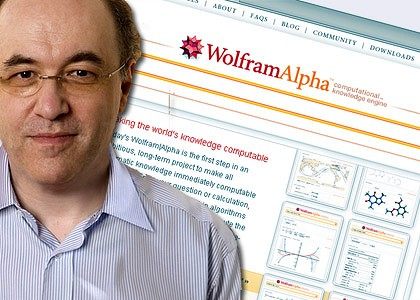
\includegraphics[width=\linewidth]{pict/alpha}
                \end{center}
                \label{fig:alpha}
            \end{figure}
        \end{columns}
    \end{frame}

    \begin{frame}
        \frametitle{Нульмерный автомат}
        \begin{columns}[c] % the "c" option specifies center vertical alignment
            \column{.45\textwidth} % column designated by a command
            Состояние ячейки во время временного шага \(i\) является целым числом, \(x_i\). В качестве начального условия предположим, что \(x_0 = 0\). Ячейка может иметь только одно из двух состояний: 0 или 1. Для клеточного автомата с двумя состояниями мы можем написать правило, например, \(x_{i + 1} = (x_i + 1) \% 2\), где \(\%\) – оператор деления по модулю.
            \column{.45\textwidth}
            \begin{figure}
                \begin{center}
                    
\includegraphics[width=\linewidth]{pict/zeroD}
                \end{center}
                \caption{Мигающая клетка}
                \label{fig:zeroD}
            \end{figure}
        \end{columns}
    \end{frame}

    \begin{frame}
        \frametitle{Одномерный автомат}
        \begin{figure}
            \begin{center}
                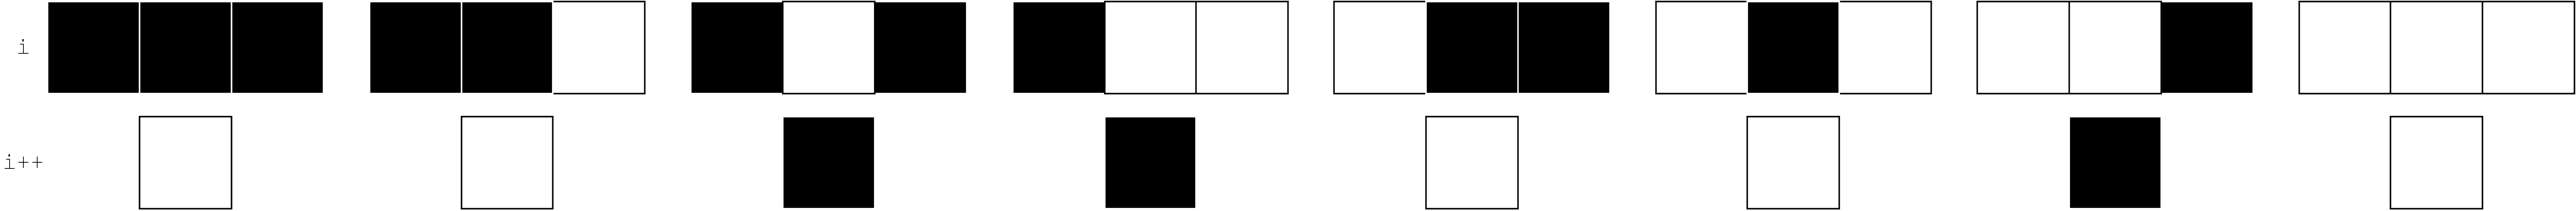
\includegraphics[width=\linewidth]{pict/rule50}
            \end{center}
            \caption{Одномерный автомат (правило 50)}
            \label{fig:rule50}
        \end{figure}
        
        \begin{table}
            \begin{center}
                \begin{tabular}{ccccccccc}
                    prev & 111 & 110 & 101 & 100 & 011 & 010 & 001 & 000\\
                    \hline
                    next &  0  &  0  &  1  &  1  &  0  &  0  &  1  &  0
                \end{tabular}
            \end{center}
            \caption{Таблица изменения состояния по правилу 50}
            \label{tab:rule50}
        \end{table}
        Расчёт количества правил производится по формуле \(2^{2^{n}}\), где \(n\) - количество клеток, влияющих на состояние.
    \end{frame}

    \begin{frame}
        \frametitle{Одномерный автомат}
        \begin{table}
            \begin{center}
                \begin{tabular}{|p{2cm}|p{2cm}|p{2cm}|p{2cm}|}
                    \hline
                    Текущее состояние & Левая клетка & Правая клетка & Следующее состояние\\
                    \hline
                    1  &  1  &  1  &  0\\
                    \hline
                    1  &  1  &  0  &  0\\
                    \hline
                    0  &  1  &  1  &  1\\
                    \hline
                    0  &  1  &  0  &  1\\
                    \hline
                    1  &  0  &  1  &  0\\
                    \hline
                    1  &  0  &  0  &  0\\
                    \hline
                    0  &  0  &  1  &  1\\
                    \hline
                    0  &  0  &  0  &  0\\
                    \hline
                \end{tabular}
            \end{center}
            \caption{Таблица изменения состояния по правилу 50}
            \label{tab:rule50logic}
        \end{table}
    \end{frame}

    \begin{frame}
        \frametitle{Одномерный автомат}
        \begin{figure}
            \begin{center}
                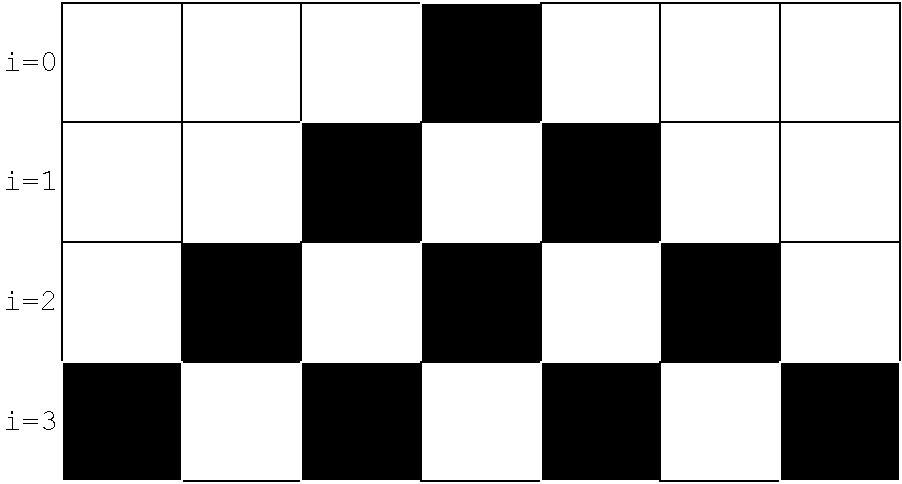
\includegraphics[width=\linewidth]{pict/oneD50}
            \end{center}
            \caption{Одномерный автомат (правило 50) во времени}
            \label{fig:oneD50}
        \end{figure}
    \end{frame}

    \begin{frame}
        \frametitle{Одномерный автомат}
        \begin{table}
            \begin{center}
                \begin{tabular}{ccccccccc}
                    prev & 111 & 110 & 101 & 100 & 011 & 010 & 001 & 000\\
                    \hline
                    next &  0  &  0  &  0  &  1  &  0  &  0  &  1  &  0
                \end{tabular}
            \end{center}
            \caption{Таблица изменения состояния по правилу 18}
            \label{tab:rule18}
        \end{table}

        \begin{table}
            \begin{center}
                \begin{tabular}{|p{2cm}|p{2cm}|p{2cm}|p{2cm}|}
                    \hline
                    Текущее состояние & Левая клетка & Правая клетка & Следующее состояние\\
                    \hline
                    1  &  1  &  1  &  0\\
                    \hline
                    1  &  1  &  0  &  0\\
                    \hline
                    0  &  1  &  1  &  0\\
                    \hline
                    0  &  1  &  0  &  1\\
                    \hline
                    1  &  0  &  1  &  0\\
                    \hline
                    1  &  0  &  0  &  0\\
                    \hline
                    0  &  0  &  1  &  1\\
                    \hline
                    0  &  0  &  0  &  0\\
                    \hline
                \end{tabular}
            \end{center}
            \caption{Таблица изменения состояния по правилу 18}
            \label{tab:rule18logic}
        \end{table}
    \end{frame}

    \begin{frame}
        \frametitle{Одномерный автомат}
        \begin{figure}
            \begin{center}
                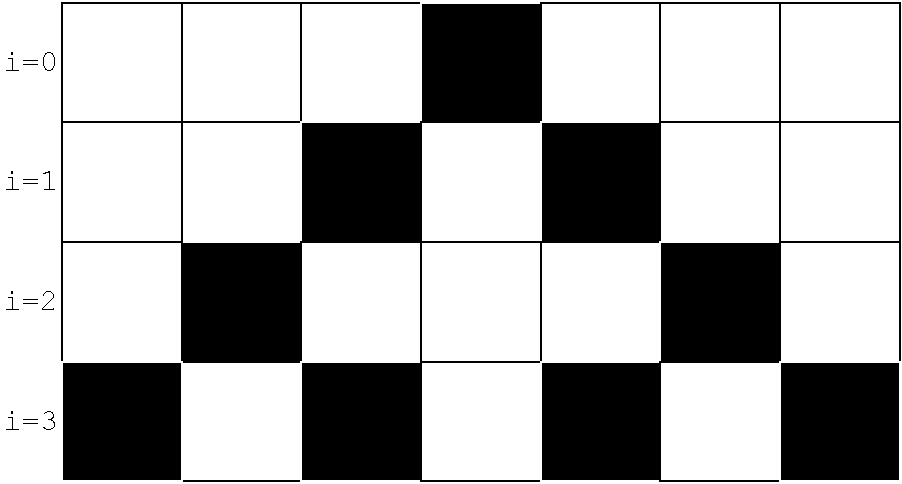
\includegraphics[width=\linewidth]{pict/oneD18}
            \end{center}
            \caption{Одномерный автомат (правило 18) во времени}
            \label{fig:oneD18}
        \end{figure}
    \end{frame}

    % \begin{frame}[allowframebreaks]
    %     \frametitle{Список литературы}
    %     \printbibliography
    % \end{frame}

\end{document}